\chapter{Methodology}
\label{ch:methodology}


\section*{Architecture}
\label{ch:architecture}

The architecture of the developed software was developed with the requirements in \autoref{ch:requirements} in mind.
The following section will explain how the individual additions to the existing code are designed and why the design was chosen.


\subsection[]{Tabular Processor}
\label{ch:architecture-tabularProcessor}

To allow for a flexible use and the possibility to add additional processing mechanism, the strategy design pattern (\autoref{fig:design}) was chosen \cite{gamma1994design}.
The pattern is especially useful, if a certain behavior is required but needs to be realized in different ways.
The Strategy defines what kind of methods need to be implemented and the concrete implementations, the different strategies, implement the behavior in different ways.
Depending on the context, different strategies can be used interchangeably, since all implemented the same functionalities.
Additionally, new strategies can be added easily without affecting any of the other strategies or the context \cite{gamma1994design}.

\begin{figure}[h]
	\centering
	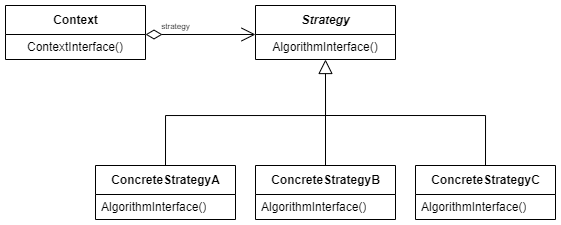
\includegraphics[width=0.8\textwidth]{images/strategy.png}
	\caption{Strategy Pattern \cite[p. 316]{gamma1994design}}
	\label{fig:design}
\end{figure}

\begin{figure}[h]
	\centering
	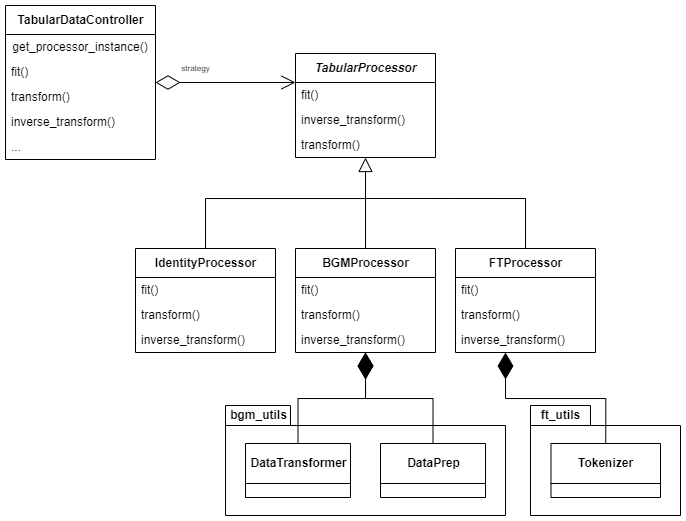
\includegraphics[width=0.8\textwidth]{images/tabular_processor.png}
	\caption{Tabular Processor Design}
	\label{fig:tabular_processor}
\end{figure}

\autoref{fig:tabular_processor} shows how the strategy pattern is realized.
The overall Strategy is defined in the TabularProcessor class in the form of an abstract class with three core methods, each tabular processing mechanism needs to implement.
These functions are the fit, transform and inverse transform functions (FR[TODO]- FR[TODO]).

Each different tabular processing strategy is different and realizes the transformation of the data in a different way by implementing the abstract classes of the parent strategy.
Therefore, Additional tabular processing mechanism can be easily added, by just implementing the abstract methods (FR[TODO]).
Furthermore, the tabular processing mechanism can be exchanged easily, since they share the same functions.
This is handled in the TabularDataController class, which equivalent to the Context in the Strategy Pattern.
The TabularDataController handles all relevant aspects in order to use the tabular processing mechanisms, including but not limited to the instantiation, fitting, saving and loading of tabularProcessor instances.
To instantiate a tabular processor, the data separated into categorical, numerical and target as numpy-arrays \cite{harris2020array} need to be provided.
The first step in using the tabular processor is fitting it according to the data.
Additional required information for fitting can be provided through meta-data in the form of a dictionary.
Note that this fit function might not be necessary, depending on the processing mechanism, however, it should be implemented anyways.
Only after fitting, the transform function can be called, transforming the data and returning the transformed data in the same format.
The inverse transformation works in the same way, but just reversing transformed data back into its original format.


\subsection[]{Tabular Processor Implementations}
\label{ch:architecture-tabularProcessor-implementations}

Three different tabular processor versions have been implemented.
The IdentityProcessor, does not do anything to the data.
It is used to do experiments without any tabular processing mechanism.

\subsubsection*{BGMProcessor}
\label{ch:BGMProcessor}

The BGMProcessor is the same processing mechanism that has been introduced by the CTABGAN+ model \cite{zhao2022CTABGANEnhancingTabular}.
Firstly, a mixed-type encoding is introduced, specifically designed to encode single columns that contain both, numerical and categorical data types.
For the continues values, the authors adapt the mode-specific normalization technique from \cite{xu2019ModelingTabularData} using a \gls{bgm} implementation \cite{BayesianGaussianMixture}, which is a \gls{vgm} (see \autoref{sec:dataNormalization} for details).
For the categorical values, the $\beta$ one-hot vector is extended the number of possible categorical values in the column.
If a categorical value should be encoded, the $\alpha$ value is set to 0 and the one-hot encoding indicating the specific category is set to 1.
Additionally, the authors allow missing values, which are treated as another categorical entry.
Furthermore, the authors introduce a "general transform" mechanism \cite[p. 7]{zhao2022CTABGANEnhancingTabular} that is supposed to be used for simple distributions and counters the problem of exploding dimensionality caused by a one-hot encoding \cite{zhao2022CTABGANEnhancingTabular}.
This general transformation is mapping of the value into a range of  [-1, 1], that is achieved through a shifted and scaled min-max normalization (see MinMaxScaler in \autoref{sec:dataNormalization}).
Mathematically, the encoded datapoint $x^t_i$ can be computed using the original datapoint $x_i$ in column $x$ through the following formula:
$$x^t_i=2* \frac{x_i-\min(x)}{\max(x)}-\min(x)-1$$
which can easily be reversed with:
$$X_i = (\max(x)-\min(x))*\frac{X^t_i+1}{2}+\min(x)$$
Categorical values are label encoded before applying the normalization \cite{zhao2022CTABGANEnhancingTabular}.
The authors observe, that this simplistic general transformation for continuos values only works well for simple distribution (\eg single-mode gaussian) and not for complex distributions, for which the mode-spefic normalization is preferred \cite{zhao2022CTABGANEnhancingTabular}.
For categorical values, the general transformation should only be applied if the number of categories a column can take is very high and would lead to very sparse vectors that make computation difficult \cite{zhao2022CTABGANEnhancingTabular}.
Lastly, the authors log-transform columns that suffer from very long-tails (see \autoref{sec: synthetic tabular data generation}), because \Glspl{bgm} seem to have difficulties to encode values towards the tail \cite{zhao2022CTABGANEnhancingTabular}.
The log-transformation of each value $\tau$ in the column will be compressed to $\tau^e$, given a lower bound $l$ using:
\begin{equation}
	\label{eqn:log-transform}
	\begin{align*}
		\tau^e =
		\begin{cases}
			log(\tau)            & \text{if} l>0                                 \\
			log(\tau-l+\epsilon) & \text{if} l\leq0 \text{, where } \epsilon > 0
		\end{cases}
	\end{align*}
\end{equation}

This encoding strategy is realized in the BGMProcessor class, that uses the DataPrep and DataTransformer class, as developed by \cite{zhao2022CTABGANEnhancingTabular}.
These classes require additional information about the dataset, provided by the user, including what columns are categorical, categorical columns that have a high cardinality/dimensionality\footnote[]{Inside the code of the authors, they refer to it as "non_categorical_columns", which is a bit misleading. Categorical columns with high dimensionality are transformed to numerical columns and handled as if they were continuous.}, numerical, mixed (including what values are categorical) as well as what columns require a log-transformation and which a general transformation.
Inside the Tabular Processor, this is realized by extending the info.json (\autoref{lst:info}) with an additional entry, dataset\_config [TODO: Kursiv?], see \autoref{lst:info_extended} for an example.

\begin{lstlisting}[label={lst:info_extended},caption={Example extended data info file}]
    {
    "name": "Adult",
    [...]
    "val_size": 6513,
    "dataset_config": {
        "cat_columns": [ // categorical columns
            "workclass", 
            (...), 
            "income"
            ],
        "non_cat_columns": [], // high dim-categorical
        "log_columns": [], // log-transformation
        "general_columns": [ //  general-transformation
            "age"
            ], 
        "mixed_columns": { // mixed-data-types
            "capital-loss": [0.0], // the "0.0" value is categorical           
            "capital-gain": [0.0]
            },
        "int_columns": [ // numerical columns 
            "age", 
            (...), 
            "hours-per-week"
        ],
        "problem_type": "binclass", // [binclass|multiclass|regression]
        "target_column": "income"
        }
    }
\end{lstlisting}

\subsubsection*{FTProcessor}
\label{ch:FTProcessor}

The FTProcessor, short for \gls{ft} Processor, is based upon the work of \cite{zheng2022DiffusionModelsMissing, gorishniy2021RevisitingDeepLearning}.
The \gls{ft} transforms tabular data into a static embedding representation.
Categorical columns are embedded through an Embedding layer, which is basically a look up table \cite{EmbeddingPyTorch13} of fixed size.
Each categorical input tensor of dimensions $[N]$ will be transformed in an embedding of size $[N,H]$ with $H$ as the embedding dimensionality \cite{gorishniy2021RevisitingDeepLearning}.
Numerical columns will be processed by a simple multiplication of a linear layers weights \cite{gorishniy2021RevisitingDeepLearning}.
Lastly, a bias term is added to both categorical and numerical columns.
\autoref{fig:ft} illustrates how a tabular data row with tree numerical and two categorical features could be transformed into a new tensor \cite[Figure 2a, p.4]{gorishniy2021RevisitingDeepLearning}.

\begin{figure}[h]
	\centering
	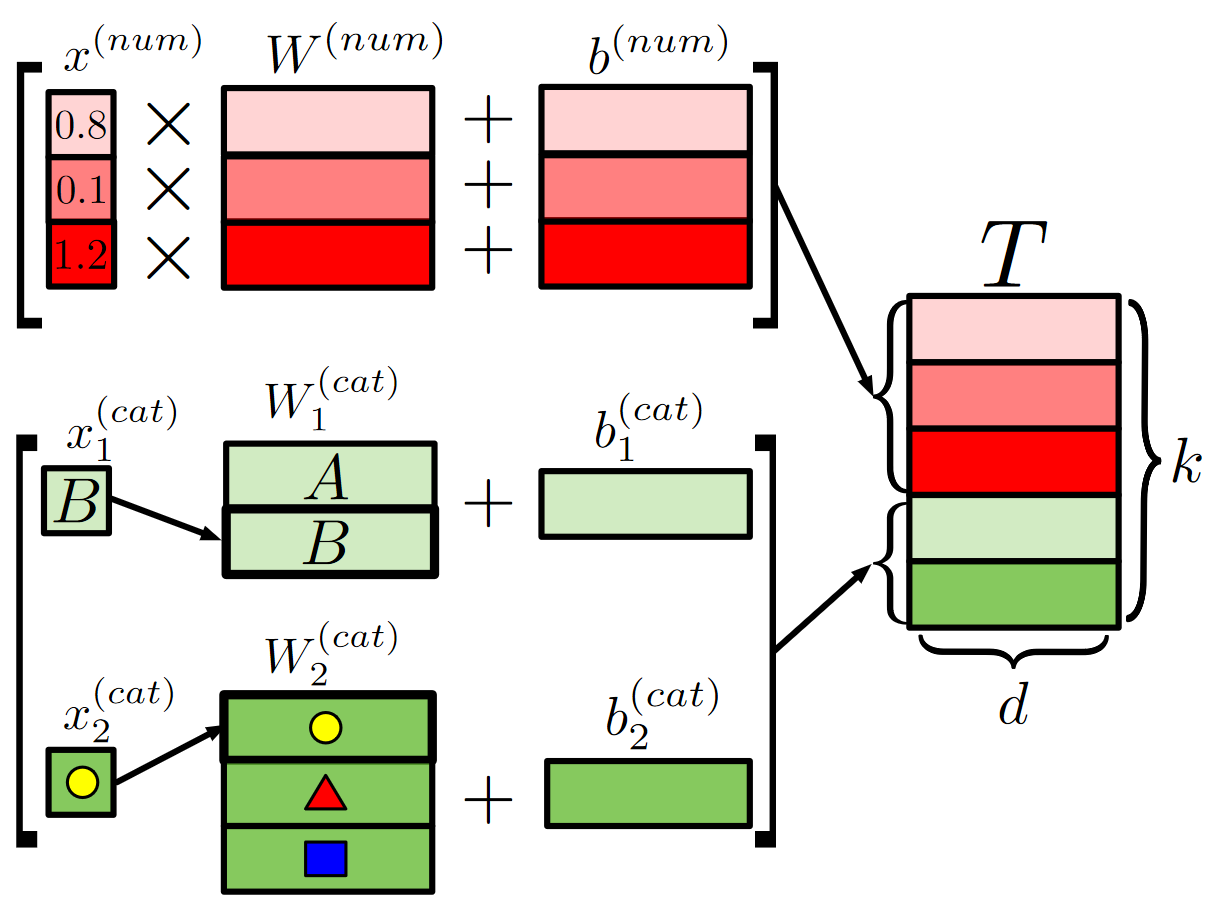
\includegraphics[width=0.5\textwidth]{images/ft.png}
	\caption{Feature Tokenization \cite[Figure 2a, p.4]{gorishniy2021RevisitingDeepLearning}}
	\label{fig:ft}
\end{figure}

To revert the data that are produced by the diffusion model to the original data format, the numerical and categorical columns need to be handled differently.
Numerical output is divided element-wise by the corresponding embedding weights and the average value is computed, as the final output\cite{zheng2022DiffusionModelsMissing}.
For categorical output, the closest categorical embedding is determined by computing the euclidean distance between the produced output and every categorical embedding \cite{zheng2022DiffusionModelsMissing}.

While in the original work of \cite{gorishniy2021RevisitingDeepLearning}, the feature tokenizer is directly in front of a transformer model, allowing the gradients to flow through the embedding and linear layers during training.
This enables the model to learn a meaningful embedding.
In the adaptation of \cite{2023DiffusionModelsMissing} and in this thesis, the weights of the layers are frozen, hence, learning is not possible and the embedding is static.
In this thesis, the data transformation and the actual model training are fully separated, hence, gradients can not flow back to the feature tokenizer to update any weights of the embeddings.


\section{Experimental Setup}
\label{ch:methods-experimentalSetup}

The code was developed in python version 3.9.7 and made use of several libraries.
A full list can be found in [TODO:].

The training was performed using Microsoft Azure Machine Learning Studio.
Each experiment was executed on an STANDARD_NC6 compute cluster running on linux, consisting of six virtual \glspl{cpu} (Intel Xeon E5-2690v3) with 56 GB Memory, 340 GB (SSD) Storage and the computing of one-half \gls{gpu} (Tesla K80) with 12 GB \gls{gpu} memory \cite{msft2022NCseriesAzureVirtual}.

The hyperparameter search space for the various models was not changed and is equal to the experiments in \cite{kotelnikov2022TabDDPMModellingTabular} and .
\begin{table}[h]
	\centering
	\begin{tabular}{l | l }
		\hline
		Parameter                 & Distribution        \\
		\hline
		Max depth                 & UniformInt[3, 10]   \\
		Learning rate             & LogUniform[1e-5, 1] \\
		Bagging temperature       & Uniform[0,1]        \\
		L2 leaf reg               & LogUniform[1,10]    \\
		Leaf estimation iteration & UniformInt[1,10]    \\
		\hline
		Number of tuning trials   & 100
	\end{tabular}
	\caption{CatBoost evaluation model hyperparameter tuning search space (proposed by \cite{gorishniy2021RevisitingDeepLearning})}
	\label{tab:catboost_tune}
\end{table}

\begin{table}[h]
	\centering
	\begin{tabular}{l | l }
		\toprule
		Parameter               & Distribution                       \\
		\midrule
		Learning Rate           & LogUniform[1e-5,3e-3]              \\
		Batch Size              & Cat\{256,4096\}                    \\
		Diffusion timesteps     & Cat\{100,1000\}                    \\
		Training iterations     & Cat\{5000,10000,20000\}            \\
		\# MLP layers           & Int\{2,4,6,8\}                     \\
		MLP layer width         & Int\{128,256,512,1024\}            \\
		Proportion of samples   & Float\{0.25, 0.5, 1, 2\}           \\
		\midrule
		Train size              & \#entries in training dataset      \\
		\# Samples              & Proportion of samples * Train size \\
		Dropout                 & 0.0                                \\
		Scheduler               & cosine                             \\
		Gaussian diffusion loss & mse                                \\
		\bottomrule
		Number of tuning trials & 100
	\end{tabular}
	\caption{TabDDPM model hyperparameter tuning search space}
	\label{tab:diff_tune}
\end{table}



\begin{table}[h]
	\centering
	\begin{tabular}{l | l }
		\hline
		Parameter               & Distribution                     \\
		\hline
		\# classif. layers      & UniformInt[1,6]                  \\
		Classif. layer size     & Int\{62, 128, 256, 512\}         \\
		Training itertations    & Cat\{5000, 20000, 30000\}        \\
		Batch size              & Cat\{456,4096\}                  \\
		Embedding dim.          & Int\{16,32,64,128,256,512,1024\} \\
		Loss factor             & LogUniform[0.01, 10]             \\
		Proportion of samples   & Float\{0.25, 0.5, 1, 2, 4, 8\}   \\
		\hline
		Number of tuning trials & 100
	\end{tabular}
	\caption{TVAE model hyperparameter tuning search space}
	\label{tab:tvae_tune}

\end{table}

\begin{table}[h]
	\centering
	\begin{tabular}{l | l }
		\hline
		Parameter               & Distribution                   \\
		\hline
		\# classif. layers      & UniformInt[1,4]                \\
		Classif. layer size     & Int\{62, 128, 256\}            \\
		Training itertations    & Cat\{1000, 5000, 7500\}        \\
		Batch size              & Int\{512,1024,2048\}           \\
		random dim.             & Int\{16,32,64,128\}            \\
		\# Channels             & Int\{16, 32, 64\}              \\
		Proportion of samples   & Float\{0.25, 0.5, 1, 2, 4, 8\} \\
		\hline
		Number of tuning trials & 30
	\end{tabular}
	\caption{CTAGBAG/CTABGAN+ model hyperparameter tuning search space. Training iterations and Number of tuning trails was reduced compared to the original \cite{kotelnikov2022TabDDPMModellingTabular}, to reduce computation time.}
	\label{tab:ctabgan_tune}
\end{table}

[TODO: explain the different Parameters?]


\section{Datasets}
\label{ch:methods-datasets}

The dataset that was used for experiments is the Adult dataset, also known as "Census Income" from the UCI Machine Learning repository \cite{Dua:2019}.
The dataset was constructed through an extraction from a 1994 census database \cite{kohavi1996ScalingAccuracyNaiveBayes}.
Overall, the dataset has 15 columns, of which nine are categorical and six are continuous, and 48842 rows.

The continuous columns are:

age, fnlwgt, education-num, capital-gain, capital-loss, hours-per-week

and the categorical columns are:

workclass, education, marital-status, occupation, relationship, race, sex, native-country, income

The dataset was created for binary classification, where the model should predict the column value of the income column (either ">50K" or "<=50K").

\autoref{tab:adult} shows five entries of the dataset:


\begin{table}[h]
	\centering
	\resizebox{\columnwidth}{!}{
		\begin{tabular}{|c|c|c|c|c|c|c|c|c|c|c|c|c|c|c|}
			\hline
			\textbf{age} & \textbf{workclass} & \textbf{fnlwgt} & \textbf{education} & \textbf{education-num} & \textbf{marital-status} & \textbf{occupation} & \textbf{relationship} & \textbf{race} & \textbf{sex} & \textbf{capital-gain} & \textbf{capital-loss} & \textbf{hours-per-week} & \textbf{native-country} & \textbf{income} \\ \hline
			39.0         & State-gov          & 77516.0         & Bachelors          & 13.0                   & Never-married           & Adm-clerical        & Not-in-family         & White         & Male         & 2174.0                & 0.0                   & 40.0                    & United-States           & $\leq$50K       \\ \hline
			50.0         & Self-emp-not-inc   & 83311.0         & Bachelors          & 13.0                   & Married-civ-spouse      & Exec-managerial     & Husband               & White         & Male         & 0.0                   & 0.0                   & 13.0                    & United-States           & $\leq$50K       \\ \hline
			38.0         & Private            & 215646.0        & HS-grad            & 9.0                    & Divorced                & Handlers-cleaners   & Not-in-family         & White         & Male         & 0.0                   & 0.0                   & 40.0                    & United-States           & $\leq$50K       \\ \hline
			53.0         & Private            & 234721.0        & 11th               & 7.0                    & Married-civ-spouse      & Handlers-cleaners   & Husband               & Black         & Male         & 0.0                   & 0.0                   & 40.0                    & United-States           & $\leq$50K       \\ \hline
			28.0         & Private            & 338409.0        & Bachelors          & 13.0                   & Married-civ-spouse      & Prof-specialty      & Wife                  & Black         & Female       & 0.0                   & 0.0                   & 40.0                    & Cuba                    & $\leq$50K       \\ \hline
		\end{tabular}
	}
	\caption{Adult income dataset, 5 exemplary entries}
	\label{tab:adult}
\end{table}


